\chapter{Load Balancing} \label{chapter:load_balancing}
% Non-conforming boundaries
% Say it only uses number of elements, point to results for N influence on GPUs

A well made multi-block mesh can distribute the work evenly the different worker processes without
needing runtime adjustment if the topology and areas of more expensive computation stay the same
during the whole computation. This is complicated by the fact that, as seen in
Chapter~\ref{chapter:adaptive_mesh_refinement}, the mesh elements can increase their polynomial
order and split in multiple smaller elements in areas where the solution accuracy is not estimated
to be satisfactory. Unless the regions of interest happen to be evenly distributed between the
different processes, this will lead to an imbalance as some processes are left with more elements,
or higher-order elements, within their domain.

\begin{figure}[H]
	\centering
	\subfloat[Mesh before refining]
	{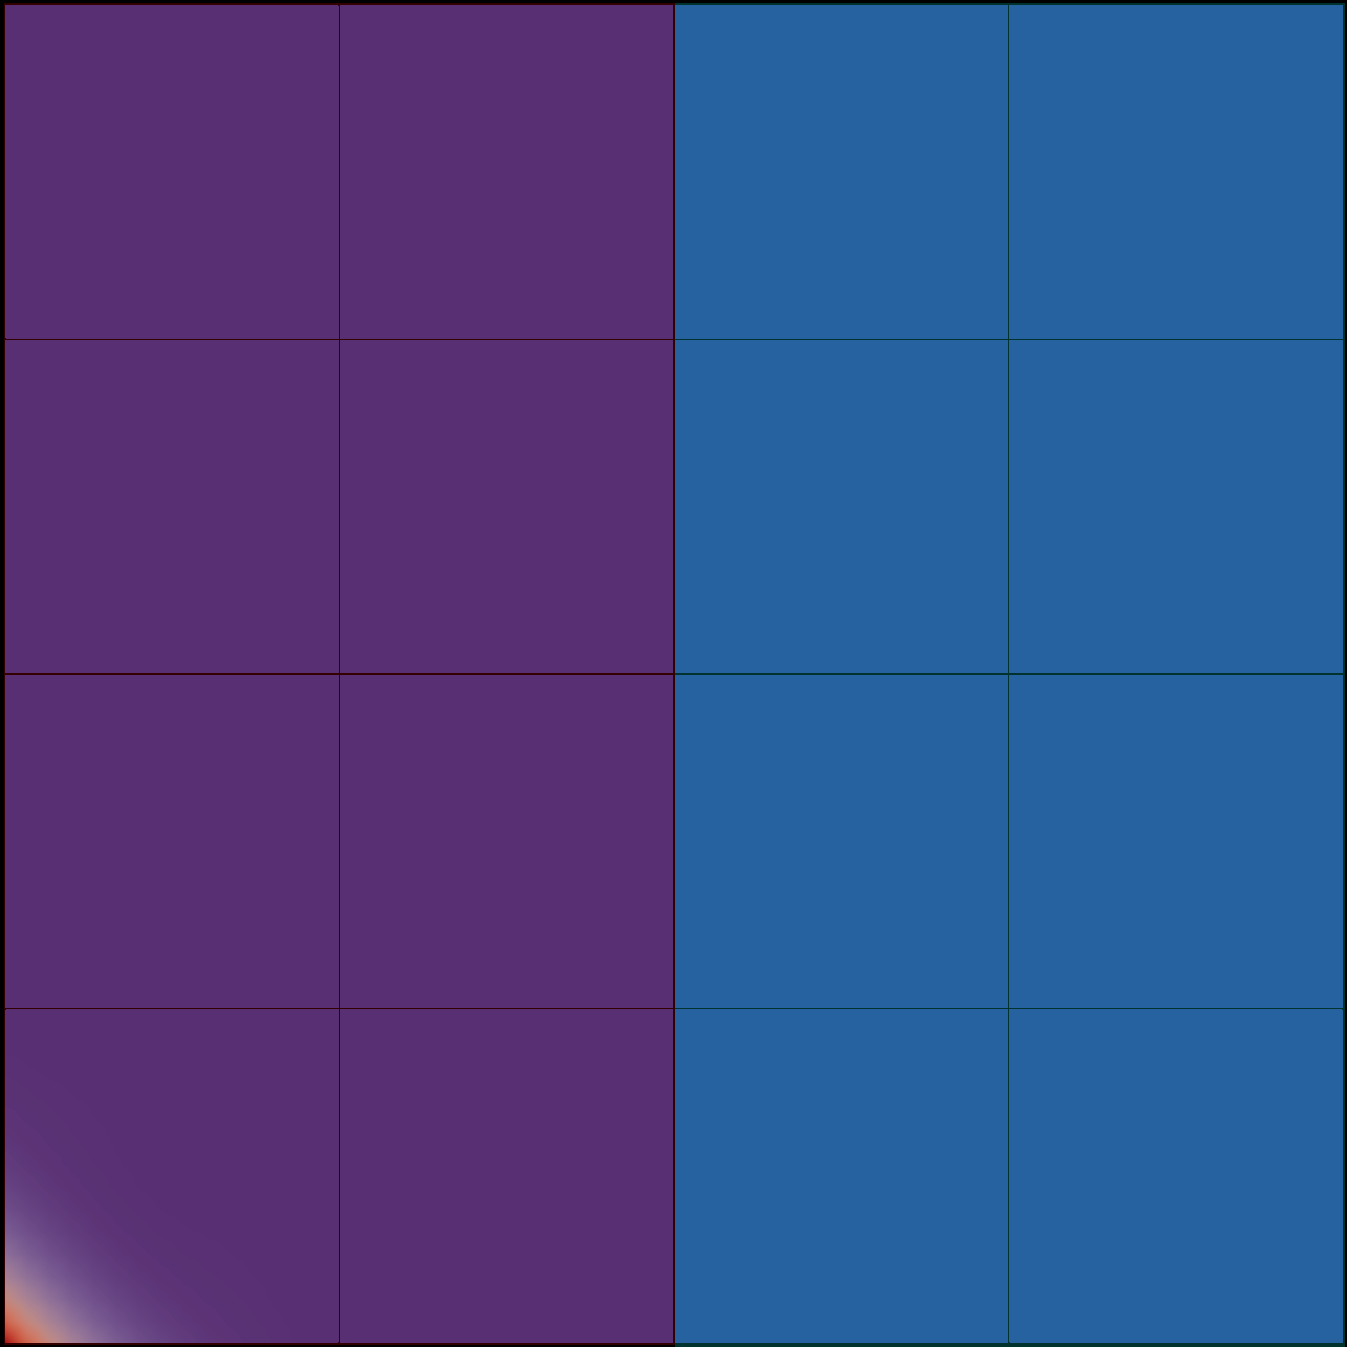
\includegraphics[width=0.45\textwidth]{Chapter_load_balancing/media/load_imbalance_initial} \label{fig:mesh_imbalance_initial_lb}}
	\hfill
	\subfloat[Mesh after refining]
	{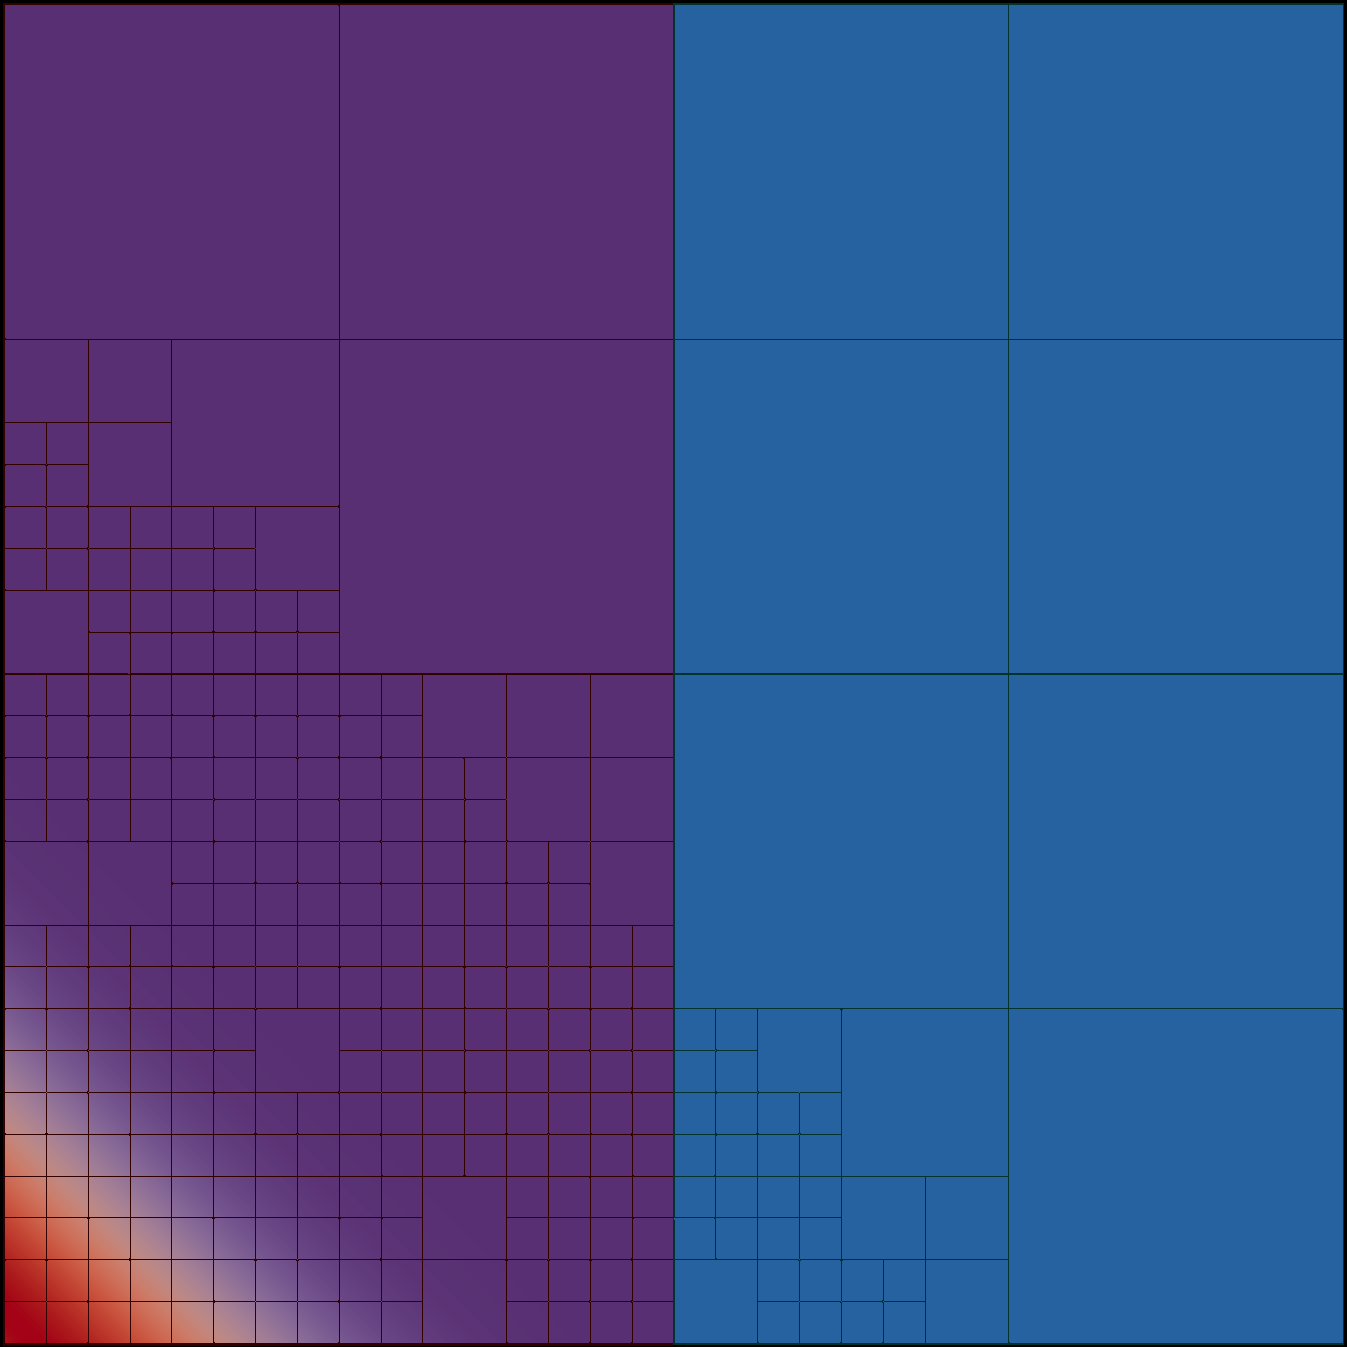
\includegraphics[width=0.45\textwidth]{Chapter_load_balancing/media/load_imbalance} \label{fig:mesh_imbalance_after_refinement_lb}}
	\caption{Load imbalance: The elements have split unequally in the two worker GPUs, one having a higher computational load. (a) Before refining (b) After refining}
	\label{fig:load_imbalance_lb}
\end{figure}

The wall time of the simulation will be driven by the most highly-loaded process, as the processes
have to synchronise at each time step. The less-loaded processes will simply wait for the other to
finish computing.

In order to keep good performance as the mesh is refined, we will need to perform dynamic load
balancing. Dynamic load balancing seeks to even out the computational load between the different
processes. The algorithm needs to be fast, to be executed often and keep the mesh optimal longer
without overshadowing the solving time. The worker processes in this work use GPUs for their
computations. Because transfers between GPUs are expensive, the algorithm needs to limit transfers
both during the load balancing process and during computation afterwards. The workers are made up of
one CPU core and one entire GPU. This means that the worker's processing power is mostly generated
by the GPU, and the algorithm needs to use it as much as possible. The algorithm will need t have
as mny parts as possible running on the GPU, in parallel. Finally, the algorithm needs to use as
little additional GPU memory as possible, as these processors have limited memory, especially
compared to CPUs.

The algorithm needs to select which elements to send from one GPU to another. Here, the
repartitioning scheme uses Space-Filling Curves (SFC), more specifically the Hilbert Curve. SFCs map
multi-dimensional space to one-dimensional space. Elements can then be sent or received from the
ends of this space. In addition, these curves are fast to generate, use low memory, and maximise
locality. Elements that are close in curve space will also be close by in the space used for
computations. This limits the number of interfaces between processes.

\section{Hilbert curve} \label{section:load_balancing:hilbert_curve}
The Hilbert curve, by D. Hilbert~\cite{Hilbert1891}, is a specific kind of space-filling curve as
described by G. Peano~\cite{Peano1890}. This curve works for 2D domains with equal and power of two
resolution in x and y. Some newer research~\cite{Haverkort2011} shows how can such curves be
expanded to three dimensions, and arbitrary domains.

\begin{figure}[H]
	\centering
	\subfloat[First level]
	{\includesvg[width=0.3\textwidth]{Chapter_load_balancing/media/hilbert_curve_K2} \label{fig:hilbert_k2}}
	\hfill
	\subfloat[Second level]
	{\includesvg[width=0.3\textwidth]{Chapter_load_balancing/media/hilbert_curve_K4} \label{fig:hilbert_k4}}
	\hfill
	\subfloat[Third level]
	{\includesvg[width=0.3\textwidth]{Chapter_load_balancing/media/hilbert_curve_K8} \label{fig:hilbert_k8}}
	\caption{Hilbert curve: The first thee Hilbert curves. (a) 2x2 (b) 4x4 (c) 8x8}
	\label{fig:hilbert_curves}
\end{figure}

Figure~\ref{fig:hilbert_curves} shows the first three levels of the Hilbert curve. The curve
successfully maps our 2D domain to a 1D one along the curve. That 1D domain can then be partitioned
between the different worker GPUs. It can be seen that the elements have good locality and no jumps. 
Wherever the curve is cut, elements on the resulting segments are close together. This is the first 
desirable propriety of the curve for this program, as we aim to reduce the contact area between 
the mesh blocks dispatched to each GPU. The iterative nature of those curves is also apparent when
put side by side. Each increasing level of the curve follows the general path of the previous curve.
Iteration is one of the possible ways to generate this curve. It will be used to generate the
initial meshes used by the program, as well as to re-number elements when the mesh refines.

\subsection{Generation} \label{section:load_balancing:hilbert_curve:generation}
We choose a table-driven algorithm to generate meshes. Each element has one of four possible states
$s$: $s \in {H, A, R, B}$. This state determines the state and ordering of the four children
elements obtained when increasing the level of the curve. The four states and their resulting
children are shown in the following figure.

% Insert figure with the four states and their results.

When put together, and assigning $H$ as the first state of the mesh, the mesh can be iteratively
constructed to the required level.

% Insert figure with the mesh from level 0 to 2

This behaviour can be summarised in the following tables. The ordering of the children elements is
from the bottom left element, in counter-clockwise order. These are implemented directly in the
code, with the state defined as an enumeration from 0 to 3 and the tables as arrays. The state
indexes into the array to get the resulting ordering and states. This gives the state $S(s, j)$ of a
cell's j\textsuperscript{th} child in function of the cell's state $s$. The same goes for the
ordering $p$ of the children, $P(s, j)$.

% Insert tables

This has the added benefit of working seamlessly in parallel, as each element can generate its
children using nothing more than its own order.

Without adaptive mesh refinement, no more work is needed. The elements wouldn't even need to store
their state, as the compact numbering of the elements is the result of the Hilbert curve. The mesh
generator included with the program works this way, creating an uniform power of two sized 2D mesh
numbered according to the Hilbert curve. The mesh generator uses the standard CGNS format. The
meshes generated this way can be used directly by the program on a single GPU, or split into
multiple blocks using the provided mesh partitioner. The mesh partitioner can split any single-block
CGNS mesh into a multi-block mesh, which can then be run using the main program on multiple GPUs.

\subsection{Refinement} \label{section:load_balancing:hilbert_curve:refinement}
% Initial guess
% Need initial guess because meshes don't store state, can be generated however
% How adaptivity uses state
% How it works well in parallel, prefix sum etc


\section{Reconstruction} \label{section:load_balancing:reconstruction}
% Having no state
% What is sent

\section{Implementation} \label{section:load_balancing:implementation}
\subsection{Element exchange} \label{section:load_balancing:implementation:element_exchange}
% and MPI datatype
% ghost elements numbering